\paragraph{}{
	Le banc de registres constitue la mémoire du processeur. Il possède
	16 registres d'un octet. Un tel circuitn 	est composé de bascules
	D en cascade. Il y en a une pour chaque registre. Il est à la figure
	\ref{banc_reg_circ}. \newline
	L'écriture d'un registre est possible uniquement lorsque \textit{regWrite}
	est à vrai.
}

\begin{figure}
	\centering
	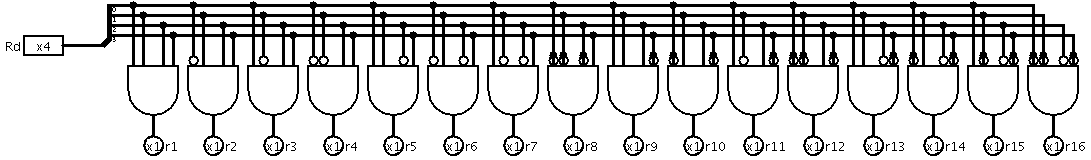
\includegraphics[scale=0.4,angle=90,origin=c]{circuits/banc_reg.png}
	\caption{
		\label{banc_reg_circ}
		Sch\'{e}ma \'{e}lectronique pour le banc de registres
	}
\end{figure}

	\subparagraph{Sélecteur de registres}{
		Attention, le sélecteur à la figure \ref{banc_reg_selec_circ}, n'est
		pas le même que le sélecteur de registres présenté en amont.
		Celui-ci est spécifique au banc de registres. C'est le circuit
		\textit{BC selec Reg} sur le schéma à la figure \ref{banc_reg_circ}.
	}

\begin{figure}
	\centering
	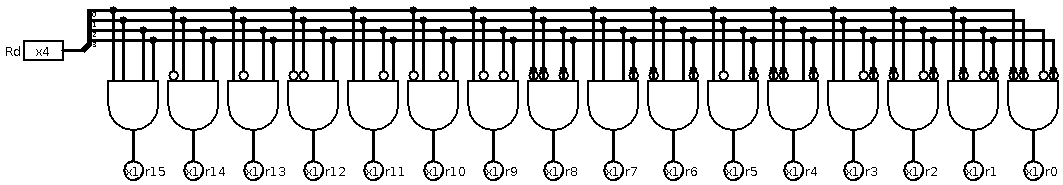
\includegraphics[scale=0.3,origin=c]{circuits/banc_reg_selec.png}
	\caption{
		\label{banc_reg_selec_circ}
		Sch\'{e}ma \'{e}lectronique pour le sélecteur du banc de registres
	}
\end{figure}